% fs document setup
\documentclass[13pt]{amsart}
% \documentclass[useAMS,usenatbib]{mnras}
\usepackage[margin=0.75in]{geometry} % see geometry.pdf on how to lay out the page. There's lots.
\geometry{a4paper} % or letter or a5paper or ... etc
% \geometry{landscape} % rotated page geometry
\usepackage{amsmath}
%\PassOptionsToPackage{pdfpagelabels=false}{hyperref}
%\usepackage[figure,figure*]{hypcap}
\usepackage[dvipsnames]{xcolor}
\usepackage{graphicx}
\usepackage{float}
\usepackage{subcaption}
\usepackage{url}
%\usepackage[font=small,labelfont=bf]{caption} % Required for specifying captions to tables and figures

% See the ``Article customise'' template for come common customisations

\title{Term Project Final Report}
\author{Troy Raen}
%\date{} % delete this line to display the current date

%%--------------------------------------------------------------------
% MACROS
% \newcommand{\Msun}{\mathrm{M}_{\odot}} % Msun/h
% \newcommand{\hw}[1]{{\color{TealBlue}[HW #1]}}
% \newcommand{\Q}[1]{{\color{gray}\textbf{#1}}}
% \newcommand{\p}[2]{\vspace{5mm} \textbf{#1: }{\color{gray}\textbf{#2}}}
\newcommand{\ba}{\textbf{a}}
\newcommand{\bb}{\textbf{b}}
\newcommand{\bt}{\textbf{t}}
\newcommand{\bw}{\textbf{w}}
\newcommand{\bW}{\textbf{W}}
\newcommand{\bx}{\textbf{x}}
\newcommand{\bX}{\textbf{X}}
\newcommand{\by}{\textbf{y}}
\newcommand{\bY}{\textbf{Y}}
\newcommand{\bz}{\textbf{z}}
\newcommand{\bZ}{\textbf{Z}}

\newcommand{\equ}[1]{\[#1\]}
\newcommand{\nequ}[2]{\begin{equation}#1 \label{#2}\end{equation}}
\newcommand{\equin}[1]{\(#1\)}

\newcommand{\figscale}[4]{
% commands: width scale, path, caption, label
\begin{figure}[h]
    \centering
    \caption{#3}
    \label{#4}
    \includegraphics[width=#1\textwidth]{#2}
\end{figure}
}
%%--------------------------------------------------------------------
%%% BEGIN DOCUMENT
\begin{document}

\maketitle
%\tableofcontents

% fe document setup


\begin{abstract}
  In this work I study how the errors in photoz estimates scale with the size of the training set for various machine learning algorithms. A 'photoz' is an estimate of the redshift of a particular object (usually a star or a galaxy) that uses photometric data.
\end{abstract}


\section{Introduction and Related Work}

  It is well established that the light reaching our telescopes from distant galaxies is shifted toward the red end of the spectrum (relative to the frequency it was originally emitted at), and that the magnitude of this 'redshift' (denoted by $z$) increases with the galaxy's distance from us (e.g. see \cite{newman}, \cite{graham}, \cite{pzreview}). The combined measurements from many galaxies indicate that the universe itself, the space between galaxies, is expanding at a rate that increases with time. The precise calculation of this expansion rate is being pursued and it depends strongly on our ability to make accurate calculations/estimations of the amount by which the light from a distant galaxy is redshifted. (Actually, the calculations of all fundamental quantities in cosmology rely heavily on our ability to accurately calculate these redshifts.)

  The calculation of the redshift from measurements of light intensity generally depends on being able to find known features in the intensity as a function of frequency. Poor frequency resolution then increases the error in the redshift.

  There are two ways in which telescopes can take measurements: spectroscopy and photometry. Spectroscopy records information about the amount of light coming in over a wide range of the frequency spectrum, at high resolution. Therefore, a redshift calculated from spectroscopic measurements is very precise and can be taken as the true redshift (sometimes called a 'spec-z'). Photometry essentially divides the spectrum into a small number of bins (on the order of 5) and records only aggregated information for each bin. Thus photometry is much cheaper to do and so we have more data of this type. However, this low resolution translates into large errors on our estimates of redshift using this data. A redshift calculated in this way is called a 'photo-z'.

  Various machine learning algorithms have been used to estimate photo-z's, with neural nets and random forest regressors showing the most success (see, for example, \cite{annz2}, \cite{tpz}, and \cite{pzreview}). \textbf{In this work, I study how the errors in photo-z estimates scale with the size of the training set for selected ML algorithms.}



  \subsection{Dataset}

    I use the dataset \texttt{Catalog\_Graham+2018\_10YearPhot} (\cite{graham}) which consists of simulated telescope data (measurements in 6 photometric bins, plus errors on the measurements) for $\sim3 \times 10^6$ galaxies. The dataset includes the true redshift for each galaxy, so this is a supervised, regression problem.

    The simulated data is intended to mimic the data anticipated from the upcoming Large Synoptic Survey Telescope (LSST). LSST will collect data from large volumes of the sky and at rates several orders of magnitude above any other telescope to date. The community is making large efforts towards dealing with data at this scale, and one of these efforts is toward quick and accurate photo-z calculations.

    \figscale{0.5}{../plots/figure_true_redshift_histogram.png}{Histogram of true redshifts in the dataset. True redshifts become more difficult to obtain as the redshift increases. Algorithms may have a more difficult time making accurate predictions at higher z because of the sparsity of training data.}{fig:zdist}

    \subsubsection{Features:}

      Previous algorithms have had more success using a set of transformed features commonly called 'colors'. This transformation is motivated by physics, and is done by subtracting the measurements in adjacent bins. We ensure that no information is lost in this transformation by including the raw measurement from one bin (it doesn't matter which one). So the final feature set includes 5 colors and 1 raw measurement for a total of 6 features.

      We could transform the measurement errors, via error propagation, and include them as features. The simplest way to do this is to assume the errors are uncorrelated and add them in quadrature for each color. Indeed, this is what is done in \cite{graham}. However, because of the physics at play and the way in which the measurements are taken, the errors are expected to be correlated. I have not taken the time to explore this further, but it could be pursued in future work. (Note that the GPz code requires the inclusion of errors in the feature set, see section \ref{gpz} for details).


    \begin{center}
    \begin{tabular}{|l|c|}
      \multicolumn{2}{c}{} \\ \hline
       & Correlations with Redshift \\ \hline
      redshift & 1.0 \\ \hline
      tu & \textbf{0.4551} \\ \hline
      tg & 0.1438 \\ \hline
      tr & 0.2717 \\ \hline
      ti & 0.3933 \\ \hline
      tz & 0.4234 \\ \hline
      ty & 0.4136 \\ \hline
      u10 & 0.3932 \\ \hline
      uerr10 & \textbf{0.518} \\ \hline
      g10 & 0.1435 \\ \hline
      gerr10 & 0.06651 \\ \hline
      r10 & 0.2716 \\ \hline
      rerr10 & 0.1222 \\ \hline
      i10 & 0.3931 \\ \hline
      ierr10 & 0.3822 \\ \hline
      z10 & 0.423 \\ \hline
      zerr10 & \textbf{0.4605} \\ \hline
      y10 & 0.4109 \\ \hline
      yerr10 & 0.45 \\ \hline
    \end{tabular}
    \end{center}


\section{Methodology}

  I follow \cite{newman} in evaluating the performance of ML algorithms as a function of sample size. My final results are in the form of curve fits to two statistics (detailed below) calculated on the algorithm predictions. Specifically I fit (using the Python function \texttt{scipy.optimize.curve\_fit()}) the parameters \{a,b,c\} in the function
  \equin{a+b \times N^c},
  % Use Matlab's nlinfit() to fit the function $a+b.*x.^c$
  where N is the training sample size. We are primarily interested in the value of the exponent, c. I show the results of \cite{newman} in figure \ref{fig:newman} for comparison with my results.

  The traditional metric for evaluating photo-z estimates is the scaled difference

  \nequ{\Delta z = \frac{photo_z-spec_z}{1+spec_z}.}{equ:deltaz}

  I evaluate the following two statistics on the metric:

  \nequ{\textrm{NMAD} = 1.48 \times \textrm{median}(|\Delta z|)}{equ:nmad}

  \nequ{\textrm{OUT10} = \frac{1}{N} \sum_{n=1}^N \big[ | \Delta z_n | > 0.1 \big]}{equ:out10}

  NMAD is the normalized, median absolute deviation and OUT10 is the fraction of predictions for which \equin{|\Delta z| > 10\%}. OUT10 is an important statistic because photo-z algorithms are prone to catastrophic errors in the predictions, due to both the physics involved and the inherently low resolution of photometry.

  Because I aim to evaluate and compare the performance of different algorithms (rather than any specific instance of a trained model), I train 20 models (see \ref{gpz} for exception) for each algorithm and training sample size (N) and pool the results before calculating the statistics.



  \subsection{Algorithms}

    I evaluate and compare the performance of four ML algorithms: 1) Neural Net composed of 2 hidden layers with 10 units each (NN\_2x10); 2) Neural Net composed of 3 hidden layers with 15 units each (NN\_3x15); 3) Random Forest regressor (RF) composed of bagged decision trees; and 4) GPz which is a publicly available code based on Gaussian Processes and developed specifically for photo-z's.


    \subsubsection{Neural Nets}

      I train multi-layer neural networks using two different architectures: 2x10 with 2 hidden layers, each with 10 units; and 3x15 with 3 hidden layers, each with 15 units. Both are motivated by approaches in \cite{pzreview} (see sections 4.1.1 DESDM and 4.1.2 ANNZ).

      I use the Matlab \texttt{fitnet()} function with backpropagation optimized using the Levenberg-Marquardt method. After running a few tests I set the parameters \texttt{epochs=500}, \texttt{max\_fail=50}, \texttt{min\_grad=1e-10}.
      % Due to runtime constraints, I set \texttt{epochs = 200}, \texttt{max\_fail = 100} for all training runs with Nsamples $>$ 99999.



    \subsubsection{Random Forest Regression}

      I train random forest regression models using the Matlab \texttt{fitrensemble()} function. I did some preliminary runs with \texttt{OptimizeHyperparameters='auto'} and found the following "best" options:

        \begin{table}[H]
        \begin{tabular}{ll}
          Method            & Bag \\
          NumLearningCycles & 495 \\
          MinLeafSize       & 1
        \end{tabular}
        \end{table}

        Guided by these results I tested some settings and ultimately use \texttt{Method='Bag'} with \texttt{Learners='tree'}, \texttt{MaxNumSplits=Nsamples-1}, and \texttt{NumLearningCycles = BLANK}, \texttt{Crossval = BLANK}. This generates a random forest model using BLANK decision trees, each trained on a subset of data of size N generated via bootstrap resampling.

        EXPLAIN RF REGRESSION




    \subsubsection{Gaussian Process Regression using GPz}
      \label{gpz}

      GPz is a publicly available code developed specifically for photo\_z estimates. The method is described in \cite{sgp}, and the specific code is introduced in \cite{gpz} and available at \url{https://github.com/OxfordML/GPz}. Since we studied this type of technique only briefly in the course I will outline the approach in a little more detail than I have done for NN and RF.

      A Gaussian Process (GP) is a non-parametric, non-linear, regression algorithm. It assumes output, y, is predicted by some function of the input, \bx, plus Gaussian noise \equin{\epsilon \sim N(0,\sigma^2)}:

      \equ{y = f(\bx)+ \epsilon.}

      Then the conditional probability of y given f is Normally distributed as
      \equin{p(y|f) \sim N(f,\sigma^2)} and Bayes' Theorem can be used to write

      \nequ{p(f|y,\bX) = \frac{p(y|f) p(f|\bX)}{p(y|\bX)}}{equ:cond}

      The prior, \equin{p(f|\bX)}, is modeled non-parametrically using kernels that model the density around each input point. GPz uses radial basis functions for these kernels. Standard GP models are computationally expensive since there is a kernel for each datapoint and the solution requires us to invert an NxN covariance matrix associated with the kernels. GPz dramatically reduces the complexity by using sparse kernels and maintains performance by optimizing hyperparameters (governing the shape and length scale) that are unique to each kernel rather than standard, global hyperparameters. This allows kernels to specialize on different regions of parameter space, and this flexibility is cited as a key reason for the success of GPz (see \cite{sgp} for a detailed derivation).

      GPz also has a large component that is focused on modeling the input noise and estimating the variance in the prediction due to two factors, the input noise and uncertainty due to the density of training points in a particular region. 'True' redshifts are more difficult to obtain at higher redshifts, and so the training data is not uniformly sampled (see Figure \ref{fig:zdist}) However, I only use the point estimate of (\ref{equ:cond}) in this work, so I will not describe the error calculations.

      GPz performs regression to optimize the hyperparameters, and in this process it explicitly minimizes the absolute value of the metric itself
      (\equin{| \Delta z |})
      rather than something more common like the mean squared error.

       % performs Bayesian analysis of L(y|w) = . It uses a sparse kernel method . Sparsity is obtained by assigning to each kernel unique hyperparameters governing its shape separate, rather than the global hyperparameters of standard kernel methods. This allows it to use a much smaller number of kernels while retaining predictive power.

      % non-parametric, probabilistic model that assumes output is predicted by some function of the input plus Gaussian noise. Uses kernel basis functions phi (specifically, the radial basis function) to model the density around a given data point. Does Bayseian analysis with likelihood = p(y|w) = ~N(mean=phi*w, sigma propto uncertainty due to density of training points in the region (=> uncertainty in mean prediction) + noise or error in the nearby input datapoints (heteroscedastic incorporated here)), prior = ?. Gives a posterior conditional , from which I take the point estimate.

      % heteroscedastic noise => errors in datapoints are correlated, in other words noise is variable and input-dependent

      % In \cite{sgp} they assert that using the sum of squares as the minimization objective function biases the metric

      % 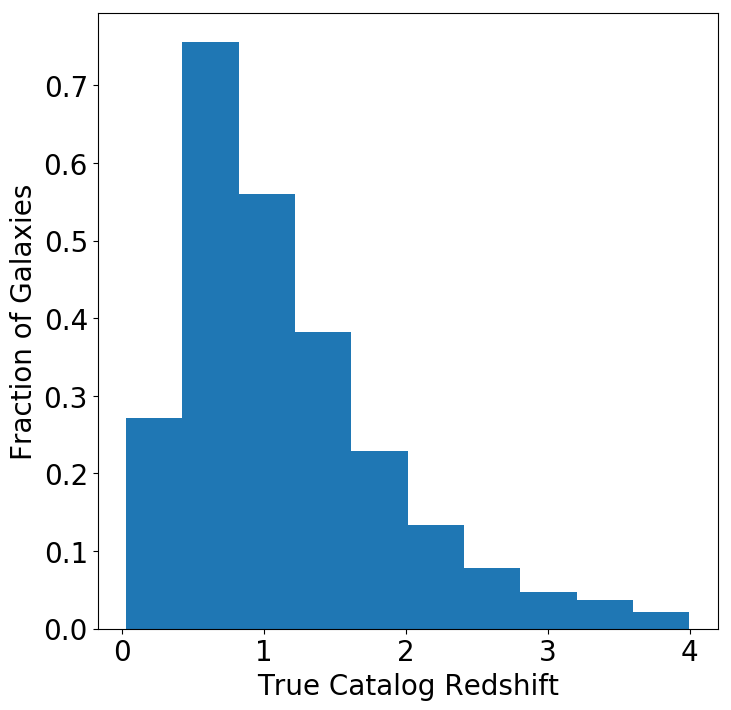
\includegraphics[width=0.5\textwidth]{../plots/figure_true_redshift_histogram.png}



\section{Experimental Results}

  The results of this work are shown in Figure \ref{fig:errs}. Figure \ref{fig:newman} shows the results of \cite{newman} for comparison.

  \figscale{1}{../data/errors_plots/errors.png}{Errors in photo-z estimates as a function of training set size for selected ML algorithms.}{fig:errs}

  \figscale{1}{../proposal/photozerrors.png}{Reproduced from Newman et al., 2019 (\cite{newman})}{fig:newman}




\section{Analysis of Results and Discussion}

  Requires the use of the measurement errors, so these models use more information than the NN or RF cases. GPz performs the feature transformation internally, so the feature inputs to this algorithm are the raw measurements, including the errors.

  TRY VARYING m, THE NUMBER OF BASIS FUNCTIONS \cite{sgp} pg 4, but plot 5 shows delta z does not vary much with training size for a given number of basis fncs => this could improve the predictions but should not change shape of scaling with N? Could bring down out10?




\section{Conclusion and Future Work}
  In \cite{gpz} they use principal component analysis to further pre-process the features, speeds up optimization.


  \subsection{Future Work}

    \begin{itemize}
      \item There is a lot of room here to tune the algorithms more finely and to test other algorithms (e.g. ANNz2, TPz). I spent several days trying to get ANNz2 running, but was unable to get it to install properly.

      \item There is also the question of why GPz performs better on the pre-packaged dataset than on the dataset I used here. Much could be explored in terms of the differences between the datasets themselves and the models learned from them.

      \item Experiment with the number of basis functions used by GPz. Find a small number (of order 5) of basis functions that still produces good predictions (must quantify 'good'). Compare these fitted kernel density estimates, and where they lie in parameter space, with two things:
        \begin{enumerate}

          \item Current physical models that predict specific types of galaxies and what their photometry measurements should look like as a function of redshift. In other words, x-type galaxies at redshift z should live in R-region of parameter space.

          \item Results of unsupervised, clustering methods which may provide insight on how many distinct types of galaxies there are as a function of redshift.
        \end{enumerate}

      \item Density estimation on the subset of the test data with out10 $>$ 10\% to see if there are localized regions of the parameter space that are not well predicted. These results could also be compared to (1) and (2) above to search for insight.

    \end{itemize}


\bibliographystyle{abbrv}
\bibliography{bib.bib}

\end{document}
